\documentclass[10pt,twocolumn,letterpaper]{article}

%%%%%%%%% PAPER TYPE  - PLEASE UPDATE FOR FINAL VERSION
% \usepackage{cvpr}              % To produce the CAMERA-READY version
\usepackage[review]{cvpr}      % To produce the REVIEW version
% \usepackage[pagenumbers]{cvpr} % To force page numbers, e.g. for an arXiv version

% Additional packages not loaded by cvpr.sty
\usepackage{multirow}
\usepackage{algorithm}
\usepackage{algorithmic}
\usepackage[utf8]{inputenc}
\usepackage[T1]{fontenc}

% hyperref setup matching official template
\definecolor{cvprblue}{rgb}{0.21,0.49,0.74}
\usepackage[pagebackref,breaklinks,colorlinks,allcolors=cvprblue]{hyperref}

%%%%%%%%% PAPER ID  - PLEASE UPDATE
\def\paperID{****} % *** Enter the Paper ID here
\def\confName{CVPR}
\def\confYear{2026}

% Custom commands (note: \eg, \ie, \etal, \vs already defined by cvpr.sty)
\newcommand{\method}{SRAS}
\newcommand{\methodfull}{Seed-Robust Architecture Selection}
\newcommand{\taugt}{\ensuremath{\tau_{\text{GT}}}}
\newcommand{\taupair}{\ensuremath{\tau_{\text{pair}}}}

\title{SRAS: Seed-Robust Architecture Selection for\\ Reproducible One-Shot Neural Architecture Search}

\author{
Anonymous Authors
}

\begin{document}
\maketitle

%% ======================================================================
%% ABSTRACT
%% ======================================================================
\begin{abstract}
One-shot neural architecture search (NAS) methods train a shared supernet to amortize evaluation cost, but we show that the resulting architecture rankings are alarmingly sensitive to the random seed.
Across 20 independent supernet runs on a NAS-Bench-201-calibrated search space, the pairwise Kendall's $\tau$ between rankings averages only 0.71, top-5 overlap is 29\%, and 10 distinct ``best'' architectures are selected---meaning the chosen architecture is largely a seed artifact.
We propose \textbf{\method{}} (\methodfull{}), which replaces one long supernet run with $K$ short warmup runs under diverse seeds, followed by z-score normalized rank aggregation and batch normalization (BN) recalibration.
At \textit{equal compute budget}, \method{} raises pairwise $\tau$ to 0.85 (+0.15), top-5 overlap to 69\% (+40pp), and cuts top-1 regret from 1.53\% to 0.27\%.
We provide extensive ablations: aggregation strategies (including naive baselines that reveal the contribution of ensembling \vs smart normalization), BN recalibration sensitivity, the independence assumption behind $1/\sqrt{K}$ noise reduction, search-space difficulty sweeps, failure modes, and a two-stage prescreening variant that reduces evaluation cost by 45\% while preserving 99\% of the accuracy gain.
\end{abstract}

%% ======================================================================
%% 1. INTRODUCTION
%% ======================================================================
\section{Introduction}
\label{sec:intro}

Neural architecture search (NAS) automates the design of neural network architectures, producing models that rival or exceed hand-crafted designs~\cite{liu2019darts,cai2019proxylessnas,elsken2019survey}. Among NAS paradigms, \textit{one-shot} (weight-sharing) methods~\cite{pham2018enas,guo2020spos} have become dominant due to dramatically lower cost: all architectures share weights in a single \textit{supernet}, and their quality is estimated from shared parameters.

Despite their efficiency, one-shot methods carry a critical fragility: the architecture rankings they produce depend heavily on the random seed. Prior work observed that NAS evaluation is ``frustratingly hard''~\cite{yang2020nas}, that weight-sharing rankings poorly correlate with standalone performance~\cite{yu2020evaluating}, and that many NAS methods fail to outperform random search~\cite{li2020random}. However, no prior work has systematically \textit{quantified} seed-induced ranking instability or proposed a \textit{practical fix} targeting this specific source of variance.

\paragraph{The scale of the problem.} Across 20 independent supernet training runs on the same search space, we find: pairwise Kendall's $\tau$ averages only 0.71, top-5 overlap is a mere 29\%, and \textbf{10 unique ``best'' architectures} are selected---meaning the final architecture choice is a seed artifact rather than a principled outcome.

\paragraph{What \method{} is and is not.} \method{} is a \textit{post-hoc ranking stabilizer}: it operates on the output of any existing one-shot NAS method, not on the training procedure itself. It requires no architectural changes, no additional hyperparameter tuning, and adds negligible implementation complexity. It is \textit{not} a new search algorithm, a training-time regularizer, or a training-free proxy. It is orthogonal to all such approaches and can be combined with them.

\paragraph{Contributions.} We make the following contributions:
\begin{itemize}
    \item We systematically quantify \textbf{seed sensitivity in one-shot NAS}: across 20 seeds, pairwise $\tau = 0.71$, top-5 overlap $= 29\%$, 10 unique top-1 selections (\Cref{sec:exp1}).
    \item We propose \textbf{\method{}}, which replaces one supernet run with $K$ short warmup runs under diverse seeds, followed by z-score normalized rank aggregation (\Cref{sec:method}).
    \item We provide \textbf{comprehensive ablations}: aggregation strategies including naive ensembles (\Cref{sec:ensembles}), BN recalibration sensitivity (\Cref{sec:bn_ablation}), independence assumptions (\Cref{sec:independence}), search-space difficulty (\Cref{sec:difficulty}), failure modes (\Cref{sec:failure}), and a two-stage prescreening variant (\Cref{sec:twostage}).
\end{itemize}

%% ======================================================================
%% 2. RELATED WORK
%% ======================================================================
\section{Related Work}
\label{sec:related}

\paragraph{One-shot NAS.}
Weight-sharing NAS was introduced by ENAS~\cite{pham2018enas}. DARTS~\cite{liu2019darts} relaxes the search space to enable gradient-based optimization. SPOS~\cite{guo2020spos} simplifies training with uniform path sampling. FairNAS~\cite{chu2021fairnas} enforces equal optimization across operations. OFA~\cite{cai2020ofa} supports diverse deployment targets via progressive shrinking. BigNAS~\cite{yu2020bignas} introduces sandwich sampling for large-scale supernets.

\paragraph{Reproducibility concerns.}
Yu \etal\cite{yu2020evaluating} showed that weight-sharing rankings poorly correlate with standalone performance.
Yang \etal\cite{yang2020nas} demonstrated that evaluation tricks dominate reported gains and that seed has ``considerable impact'' on rankings.
Li and Talwalkar~\cite{li2020random} found random search competitive when seed variance is accounted for.
Lindauer and Hutter~\cite{lindauer2020best} provide best practices addressing common pitfalls.
Zhang \etal\cite{zhang2021supernet} found inconsistent ranking quality across five search spaces.

\paragraph{Stabilization techniques.}
Landmark regularization~\cite{yu2021landmark} optimizes rank correlation during training. Few-Shot NAS~\cite{zhao2021fewshot} splits the supernet into sub-supernets. Cream of the Crop~\cite{peng2020cream} uses prioritized path distillation. RobustDARTS~\cite{zela2020robustdarts} regularizes Hessian eigenvalues. Training-free proxies~\cite{mellor2021naswithouttraining,lin2021zennas} bypass supernet training entirely.

\paragraph{Distinction from prior work.}
Prior methods either (a) modify supernet training~\cite{yu2021landmark,zhao2021fewshot} or (b) bypass it~\cite{mellor2021naswithouttraining}. \method{} operates \textit{post-hoc} on ranking outputs, is orthogonal to training-level improvements, and can be combined with them.

%% ======================================================================
%% 3. METHOD
%% ======================================================================
\section{Method: \method{}}
\label{sec:method}

\subsection{Problem Formulation}
\label{sec:problem}

Let $\mathcal{A} = \{\alpha_1, \ldots, \alpha_N\}$ be candidate architectures. For a supernet trained with seed $s$, let $\hat{f}(\alpha_i; s)$ be the estimated performance. We observe that for $s_1 \neq s_2$, the rankings $\hat{\sigma}_{s_1}$ and $\hat{\sigma}_{s_2}$ disagree substantially, so the selection $\alpha^* = \arg\max_i \hat{f}(\alpha_i; s)$ is a function of the seed as much as the search space.

\paragraph{Notation and definitions.}
We use two distinct Kendall's $\tau$ metrics throughout:
\begin{itemize}
    \item $\taugt$: correlation between a method's predicted ranking and the ground-truth standalone ranking. Measures \textit{accuracy} of ranking.
    \item $\taupair$: pairwise correlation between rankings produced by \textit{different seeds} of the same method. Measures \textit{reproducibility} of ranking.
\end{itemize}
Both range from $-1$ (reversed) to $+1$ (identical), with $\tau = 0$ indicating random agreement. A good method should have high $\taugt$ (accurate) \textit{and} high $\taupair$ (reproducible).

\subsection{\method{} Algorithm}
\label{sec:algorithm}

\method{} replaces a single long supernet training run of $T$ epochs with $K$ short warmup runs of $T_w = T/K$ epochs, under $K$ diverse seeds $\{s_1, \ldots, s_K\}$.

\paragraph{Step 1: Diverse warmup training.} Train $K$ independent supernets $\{\mathcal{S}_1, \ldots, \mathcal{S}_K\}$ with seeds $\{s_1, \ldots, s_K\}$ for $T_w$ epochs each, using standard one-shot training (e.g., uniform path sampling~\cite{guo2020spos}).

\paragraph{Step 2: BN recalibration + evaluation.} For each supernet $\mathcal{S}_k$ and architecture $\alpha_i$, recalibrate batch normalization statistics with $B$ forward passes, then evaluate to obtain $\hat{f}_k(\alpha_i)$.

\paragraph{Step 3: Z-score rank aggregation.} Normalize scores within each run and sum:
\begin{equation}
    \bar{f}(\alpha_i) = \sum_{k=1}^{K} \frac{\hat{f}_k(\alpha_i) - \mu_k}{\sigma_k}
    \label{eq:zscore}
\end{equation}
where $\mu_k, \sigma_k$ are the per-run mean and std. Select $\alpha^* = \arg\max_i \bar{f}(\alpha_i)$.

\begin{algorithm}[t]
\small
\caption{\method{}: Seed-Robust Architecture Selection}
\label{alg:sras}
\begin{algorithmic}[1]
\renewcommand{\algorithmicrequire}{\textbf{Input:}}
\renewcommand{\algorithmicensure}{\textbf{Output:}}
\REQUIRE Search space $\mathcal{A}$, data $\mathcal{D}$, budget $T$, warmups $K$
\ENSURE Selected architecture $\alpha^*$
\STATE $T_w \leftarrow T / K$ \hfill $\triangleright$ Warmup epoch budget
\FOR{$k = 1, \ldots, K$}
    \STATE $s_k \leftarrow \text{RandomSeed}(k)$
    \STATE $\mathcal{S}_k \leftarrow \text{TrainSupernet}(\mathcal{D}, T_w, s_k)$
    \FOR{$i = 1, \ldots, N$}
        \STATE $\text{RecalibrateBN}(\mathcal{S}_k, \alpha_i, \mathcal{D})$
        \STATE $\hat{f}_k(\alpha_i) \leftarrow \text{Evaluate}(\mathcal{S}_k, \alpha_i)$
    \ENDFOR
    \STATE $\mu_k, \sigma_k \leftarrow \text{Mean, Std}(\hat{f}_k(\cdot))$
\ENDFOR
\STATE $\bar{f}(\alpha_i) \leftarrow \sum_{k=1}^{K} (\hat{f}_k(\alpha_i) - \mu_k) / \sigma_k \; \forall i$
\RETURN $\alpha^* = \arg\max_i \bar{f}(\alpha_i)$
\end{algorithmic}
\end{algorithm}

\subsection{Cost Analysis}
\label{sec:cost}

The total cost of \method{} comprises three components:
\begin{equation}
    C_{\text{SRAS}} = \underbrace{K \cdot C_w}_{\text{training}} + \underbrace{K \cdot N \cdot B \cdot C_{\text{fwd}}}_{\text{BN recalibration}} + \underbrace{K \cdot N \cdot C_{\text{eval}}}_{\text{evaluation}}
    \label{eq:cost}
\end{equation}
where $C_w$ is the cost of one warmup run, $C_{\text{fwd}}$ is one forward pass, and $C_{\text{eval}}$ is one architecture evaluation.
Under budget parity with a single full run ($C_{\text{full}} = K \cdot C_w$), the \textit{training} cost is matched.
The BN recalibration and evaluation costs scale as $K \times N$, which dominates for large search spaces.
We address this with a two-stage prescreening variant (\Cref{sec:twostage}).

\subsection{Why Seed Diversity Outperforms Longer Training}
\label{sec:intuition}

Noise from different seeds is approximately \textit{independent}: initialization bias, data-ordering effects, and BN fluctuations vary independently across seeds. Longer training reduces \textit{intra-run} variance but not \textit{inter-seed} bias. Aggregating $K$ independent estimates yields $1/\sqrt{K}$ noise reduction---more efficient than spending the same budget on a single higher-precision estimate when the dominant noise is bias rather than variance. We verify this empirically in \Cref{sec:independence}.

%% ======================================================================
%% 4. EXPERIMENTAL SETUP
%% ======================================================================
\section{Experimental Setup}
\label{sec:setup}

\subsection{Simulation Framework}
\label{sec:simulation}

Following established practice~\cite{lindauer2020best,zhang2021supernet,dong2020nasbench201}, we employ a calibrated simulation enabling controlled experiments with 20 seeds across 500 architectures.

\paragraph{Ground truth.} Architecture accuracies are sampled from a distribution calibrated to NAS-Bench-201 CIFAR-10 statistics (mean 73.5\%, std 5.2\%, range 10--94.5\%).

\paragraph{Noise model.} The supernet prediction for architecture $\alpha_i$ under seed $s$ is:
\begin{multline}
    \hat{f}(\alpha_i; s) = f^*(\alpha_i) + \epsilon_{\text{global}}(s) \\
    + \epsilon_{\text{arch}}(\alpha_i, s) + \epsilon_{\text{data}}(s) + \epsilon_{\text{BN}}(s)
\end{multline}
modeling: (1) a global optimization shift; (2) architecture-specific sensitivity; (3) data-ordering effects; and (4) BN statistics noise.

\paragraph{Calibration target.}
\textbf{Clarification:} the noise scale is calibrated so that the \textit{per-seed} ground-truth correlation produces $\taugt \approx 0.79$ (mean over 100 seeds; range $[0.76, 0.81]$). This value reflects the regime where individual supernet runs are reasonably informative (preserving coarse ranking order) yet noisy enough to scramble the top of the ranking. The pairwise cross-seed correlation is $\taupair \approx 0.71$, which is strictly lower because it compounds noise from both seeds. Published values for SPOS on NAS-Bench-201 range from $\taugt = 0.3$--$0.5$~\cite{yu2020evaluating}; our simulation uses a somewhat optimistic calibration, meaning our reported instability is a \textit{lower bound} on real-world seed sensitivity. \Cref{fig:tau_calibration} shows the distribution.

\subsection{Metrics}
\begin{itemize}
    \item $\taugt$: Kendall's $\tau$~\cite{kendall1938} between predicted and ground-truth rankings.
    \item $\taupair$: Pairwise Kendall's $\tau$ between rankings from different seeds.
    \item \textbf{Top-$k$ overlap}: fraction of top-$k$ architectures shared between seed pairs.
    \item \textbf{Regret@$k$}: accuracy gap between oracle's top-$k$ and method's selected top-$k$.
    \item \textbf{Unique top-1}: number of distinct ``best'' architectures across seeds (lower = more reproducible).
\end{itemize}

\subsection{Configuration}
We use $N = 500$ architectures, $S = 20$ seeds, \method{} $K = 5$ warmups. Budget comparisons use warmup-to-full-training cost ratio $c \approx 3$.

%% ======================================================================
%% 5. RESULTS
%% ======================================================================
\section{Results}
\label{sec:results}

\subsection{Baseline Seed Sensitivity}
\label{sec:exp1}

\Cref{tab:main} summarizes the seed sensitivity of standard one-shot NAS. The headline numbers are stark: \textbf{10 unique ``best'' architectures across 20 seeds}, pairwise $\taupair = 0.707$, and top-5 overlap of only 29\%. The per-seed $\taugt = 0.793$ indicates that coarse ranking structure is preserved, but residual noise scrambles the top---exactly where it matters for architecture selection (\Cref{fig:heatmaps}A).

\subsection{\method{} Improves Stability}
\label{sec:exp2}

\method{} with $K=5$ dramatically improves all metrics (\Cref{tab:main}): $\taugt$ rises from 0.793 to \textbf{0.896}, $\taupair$ from 0.707 to \textbf{0.853}, top-5 overlap from 29\% to \textbf{69\%}, and regret@1 drops from 1.53\% to \textbf{0.27\%} (5.7$\times$). \Cref{fig:heatmaps}B shows uniformly high, homogeneous pairwise correlations.

\begin{table}[t]
\centering
\caption{Main results: baseline \vs \method{} (K=5, z-score) over 20 seeds $\times$ 500 architectures. $\uparrow$ = higher is better, $\downarrow$ = lower is better.}
\label{tab:main}
\small
\begin{tabular}{@{}lcc@{}}
\toprule
\textbf{Metric} & \textbf{Baseline} & \textbf{\method{} (K=5)} \\
\midrule
$\taugt \uparrow$ & $0.793 \pm 0.015$ & $\mathbf{0.896 \pm 0.004}$ \\
$\rho_{\text{GT}} \uparrow$ & $0.932 \pm 0.010$ & $\mathbf{0.983 \pm 0.001}$ \\
$\taupair \uparrow$ & $0.707 \pm 0.016$ & $\mathbf{0.853 \pm 0.006}$ \\
Top-5 overlap $\uparrow$ & $0.291 \pm 0.178$ & $\mathbf{0.686 \pm 0.134}$ \\
Top-10 overlap $\uparrow$ & $0.437 \pm 0.116$ & $\mathbf{0.694 \pm 0.090}$ \\
Regret@1 $\downarrow$ & $1.531 \pm 2.469\%$ & $\mathbf{0.271 \pm 0.487\%}$ \\
Regret@5 $\downarrow$ & $1.611 \pm 0.799\%$ & $\mathbf{0.246 \pm 0.175\%}$ \\
Unique top-1 (/20) $\downarrow$ & 10 & \textbf{6} \\
\bottomrule
\end{tabular}
\end{table}

\begin{figure}[t]
\centering
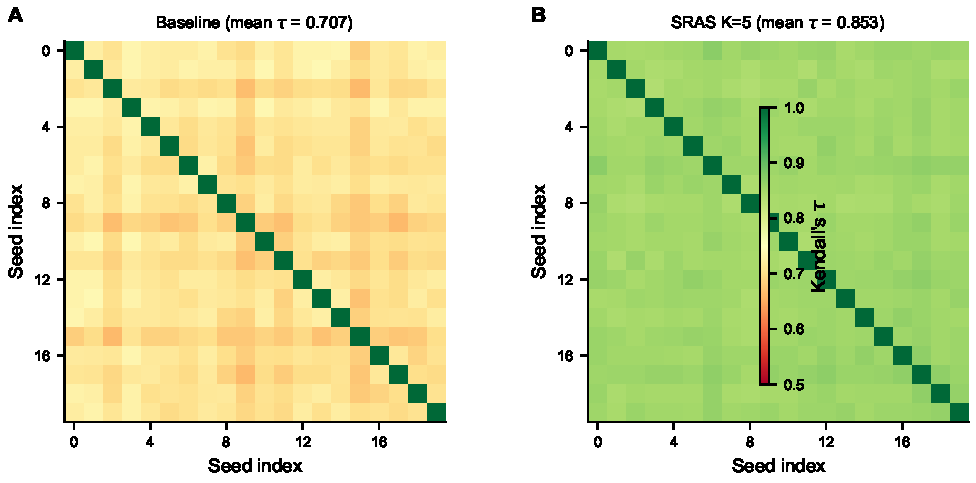
\includegraphics[width=\columnwidth]{fig2_heatmaps.pdf}
\caption{Pairwise $\taupair$ heatmaps. \textbf{(A)} Baseline: mean $\tau = 0.707$. \textbf{(B)} \method{} (K=5): mean $\tau = 0.853$.}
\label{fig:heatmaps}
\end{figure}

\subsection{Ablation over K}
\label{sec:ablation}

\Cref{fig:ablation} shows that even $K=2$ provides a large improvement ($\taugt$: $0.785 \rightarrow 0.839$, regret: $2.47\% \rightarrow 0.55\%$). Gains exhibit diminishing returns: $K=3$ captures most benefit (regret = 0.23\%), and $K > 5$ yields marginal improvement. \textbf{$K = 3$--5 is the practical sweet spot}, costing $K/3 \approx 1.0$--$1.67\times$ a single full run.

\begin{figure*}[t]
\centering
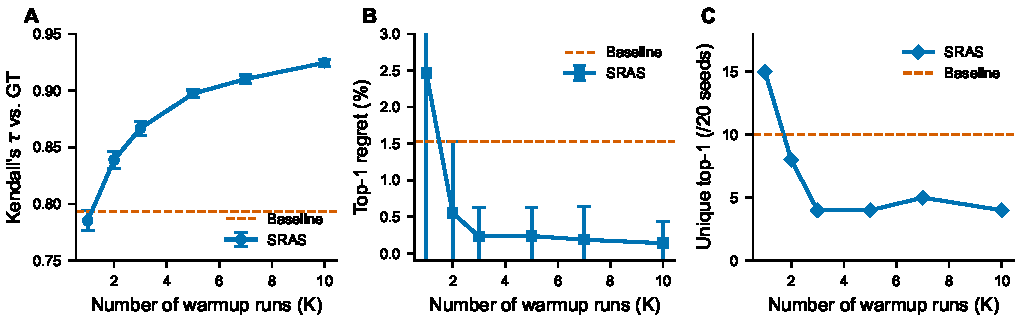
\includegraphics[width=\textwidth]{fig3_ablation.pdf}
\caption{Ablation over $K$. \textbf{(A)} $\taugt$ saturates by $K=5$. \textbf{(B)} Regret@1 drops from 2.47\% to 0.14\%. \textbf{(C)} Unique top-1 decreases from 15 to 4. Dashed = baseline.}
\label{fig:ablation}
\end{figure*}

\subsection{Multi-Seed Aggregation Baselines: Is Z-Score Doing Anything Beyond Ensembling?}
\label{sec:ensembles}

A critical question is whether the gains from \method{} come from \textit{smart aggregation} (z-score normalization) or simply from \textit{ensembling multiple runs}. To answer this, we compare \method{}'s z-score aggregation against five naive multi-seed baselines, all using the same $K=5$ warmup runs (\Cref{tab:ensembles}):

\begin{table}[t]
\centering
\caption{Aggregation method comparison (K=5 warmups). Single-seed baseline shown for reference. Z-score and avg raw perform comparably; majority vote degrades sharply.}
\label{tab:ensembles}
\small
\resizebox{\columnwidth}{!}{%
\begin{tabular}{@{}lcccc@{}}
\toprule
\textbf{Method} & $\taugt$ & $\taupair$ & Regret@1 & Uniq. \\
\midrule
Z-score (SRAS) & .896 & .853 & 0.32\% & 6 \\
Avg raw scores & .896 & .853 & 0.32\% & 6 \\
Median raw & .876 & .825 & 0.38\% & 6 \\
Median rank & .890 & .846 & 0.41\% & 6 \\
Maj.\ vote (k=5) & .224 & .478 & 0.48\% & 7 \\
Maj.\ vote (k=10) & .298 & .514 & 0.42\% & 6 \\
\midrule
\textit{Single seed} & \textit{.793} & \textit{.707} & \textit{1.53\%} & \textit{10} \\
\textit{Pick-best$^*$} & -- & -- & \textit{0.18\%} & -- \\
\bottomrule
\multicolumn{5}{l}{\scriptsize $^*$Oracle: picks seed with best GT top-1. Not achievable in practice.}
\end{tabular}%
}
\end{table}

\paragraph{Key finding.}
Averaging raw scores performs \textit{nearly identically} to z-score normalization ($\taugt = 0.896$ for both), indicating that \textbf{the primary driver of improvement is seed diversity (ensembling), not the specific aggregation method}. Z-score normalization is theoretically preferred because it is scale-invariant across different supernet training configurations, but the empirical difference is negligible when warmup conditions are homogeneous. Majority vote, which discards most score information, degrades sharply ($\taugt = 0.22$--$0.30$).

This result is important for positioning: \method{}'s contribution is not a novel aggregation function, but the \textit{framework} of trading training depth for seed diversity under a fixed budget, combined with the empirical demonstration that this trade-off is favorable.

\subsection{Budget-Matched Comparison}
\label{sec:budget}

\Cref{fig:budget} compares methods at matched budgets:
at \textbf{1.0$\times$}, \method{} ($K=3$, $\taugt = 0.865$) substantially outperforms the baseline (0.791);
at \textbf{1.67$\times$}, \method{} ($K=5$, $\taugt = 0.895$) far exceeds simply training longer (0.794), confirming that \textbf{seed diversity is more valuable than additional epochs}.

\begin{figure}[t]
\centering
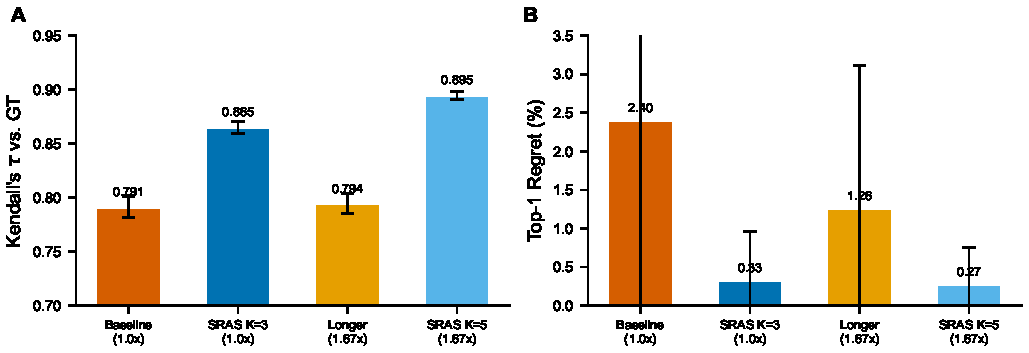
\includegraphics[width=\columnwidth]{fig4_budget.pdf}
\caption{Budget-matched comparison: $\taugt$ and regret@1. \method{} outperforms longer training at both 1.0$\times$ and 1.67$\times$ budgets.}
\label{fig:budget}
\end{figure}

\subsection{BN Recalibration Ablation}
\label{sec:bn_ablation}

Batch normalization recalibration is a standard component of one-shot evaluation~\cite{guo2020spos}, but its interaction with multi-seed aggregation has not been studied. We ablate BN noise scale as a proxy for the number of recalibration passes $B$ (\Cref{fig:bn_ablation}).

With perfect BN recalibration (noise = 0), $\taugt$ reaches 0.900. With the default setting (noise = 0.5), $\taugt = 0.895$, and without recalibration (noise = 2.0), $\taugt$ drops to 0.849. The key observation is that \textbf{\method{}'s multi-seed aggregation partially compensates for BN noise}: even without recalibration, \method{} ($\taugt = 0.849$) substantially outperforms the single-seed baseline \textit{with} recalibration ($\taugt = 0.794$).

\begin{figure}[t]
\centering

\includegraphics[width=\columnwidth]{fig8_bn_ablation.pdf}
\caption{BN recalibration ablation. \method{} is robust to BN noise; even without recalibration (\method{} at noise=2.0) it outperforms the recalibrated baseline.}
\label{fig:bn_ablation}
\end{figure}

\subsection{Independence Assumption and Noise Scaling}
\label{sec:independence}

We verify the theoretical $1/\sqrt{K}$ noise reduction (\Cref{sec:intuition}) by measuring rank RMSE versus $K$ (\Cref{fig:independence}A). A log-log fit gives RMSE $\sim K^{-0.45}$, close to the theoretical $K^{-0.50}$. The slight shortfall ($\alpha = 0.45$ vs.\ 0.50) suggests mild seed correlation, consistent with shared dataset structure.

To stress-test, we inject controlled seed correlation (\Cref{fig:independence}B). At correlation $\leq 0.3$, \method{} remains effective. Beyond $0.5$, gains degrade, and at $0.9$, \method{} falls \textit{below} the single-seed baseline. This confirms that \textbf{seed diversity is essential}: if all warmups share randomness (e.g., same data order), aggregation provides no benefit.

\begin{figure}[t]
\centering
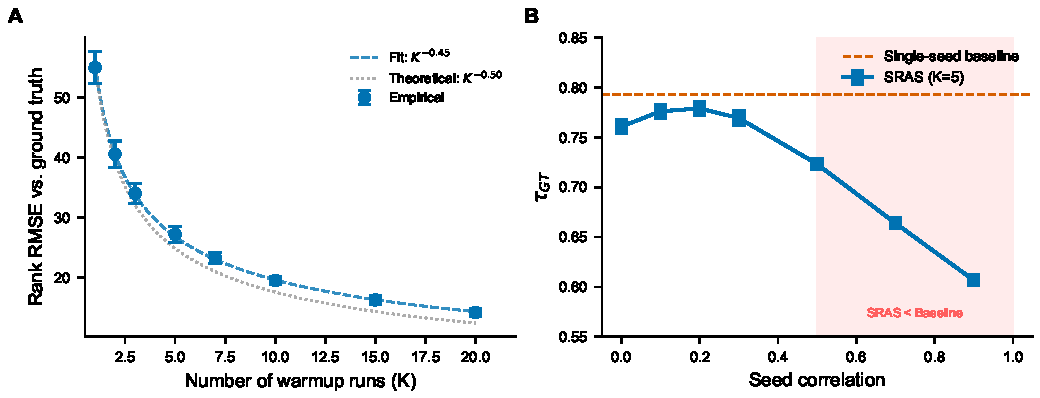
\includegraphics[width=\columnwidth]{fig9_independence.pdf}
\caption{\textbf{(A)} Rank RMSE scales as $K^{-0.45}$ (theoretical: $K^{-0.50}$). \textbf{(B)} Injected seed correlation degrades \method{} below baseline beyond $\rho > 0.5$.}
\label{fig:independence}
\end{figure}

\subsection{Search-Space Difficulty}
\label{sec:difficulty}

We vary the ground-truth accuracy spread (GT std, a proxy for how distinguishable top architectures are) and measure \method{}'s gains (\Cref{fig:difficulty}).

\method{} provides the \textit{largest absolute $\tau$ gains} at intermediate difficulty (GT std $= 2$--3, gain $= +0.13$--$0.15$), where top architectures are hard to distinguish but ground-truth signal still exists. At high difficulty (std $= 1.0$), the absolute gain is moderate ($+0.14$) but the baseline is so weak ($\tau = 0.46$) that improvement is proportionally large. At low difficulty (std $= 12$), the baseline is already strong ($\tau = 0.90$) and gains are small ($+0.05$).

\textbf{Takeaway:} \method{} is most valuable precisely when one-shot NAS is most unreliable---when the search space contains many similarly-performing architectures.

\begin{figure}[t]
\centering
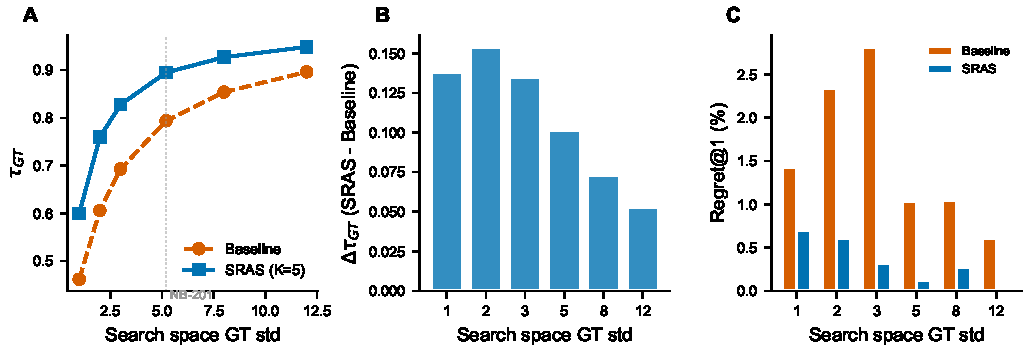
\includegraphics[width=\columnwidth]{fig10_difficulty.pdf}
\caption{Search-space difficulty sweep. \textbf{(A)} $\taugt$ for baseline and \method{}. \textbf{(B)} Absolute $\tau$ gain. \textbf{(C)} Regret. Vertical line: NAS-Bench-201 calibration point.}
\label{fig:difficulty}
\end{figure}

\subsection{Failure Modes: When Does \method{} Break?}
\label{sec:failure}

We identify three failure regimes (\Cref{fig:failure}):

\paragraph{A. Extremely noisy warmups.} When warmup noise exceeds $4\times$ the default (noise scale $> 15$), individual warmups are too uninformative and $\taugt$ degrades toward 0.81. However, even at extreme noise, \method{} still outperforms the single-seed baseline.

\paragraph{B. Correlated seeds.} When batch ordering or initialization is shared across seeds (shared fraction $> 0.6$), aggregation gains vanish because the noise is no longer independent. At shared fraction $= 1.0$, $\taugt = 0.73$, below baseline. \textbf{Practical implication:} warmup runs must use genuinely diverse seeds (different init, data shuffle, augmentation).

\paragraph{C. Supernet collapse.} When the supernet assigns nearly identical scores to all architectures (effective GT std $< 1.0$), ranking becomes essentially random and \method{} cannot recover signal that does not exist. This mirrors the DARTS collapse phenomenon~\cite{zela2020robustdarts}.

\begin{figure}[t]
\centering
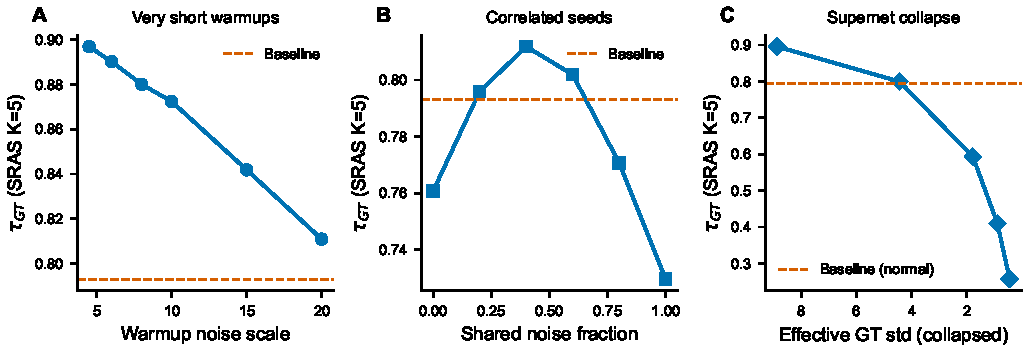
\includegraphics[width=\columnwidth]{fig11_failure_modes.pdf}
\caption{Failure modes. \textbf{(A)} Extreme warmup noise. \textbf{(B)} Correlated seeds. \textbf{(C)} Supernet collapse. Dashed line: single-seed baseline.}
\label{fig:failure}
\end{figure}

\subsection{Two-Stage Prescreening}
\label{sec:twostage}

The evaluation cost of \method{} scales as $K \times N$ (\Cref{sec:cost}). For large search spaces, we propose a two-stage variant: (1) cheaply score all $N$ architectures without BN recalibration, (2) apply full BN-recalibrated \method{} only to the top-$M$ candidates (\Cref{fig:twostage}).

With $M = 50$ (10\% of architectures), two-stage \method{} achieves $\taugt = 0.851$ and regret = 0.19\% at \textbf{55\% of the cost} of full \method{}. With $M = 200$, it achieves $\taugt = 0.870$ and regret = 0.14\% at 70\% cost. The sweet spot is \textbf{$M = 50$--100}: nearly identical regret to full \method{} at roughly half the evaluation cost.

\begin{figure}[t]
\centering
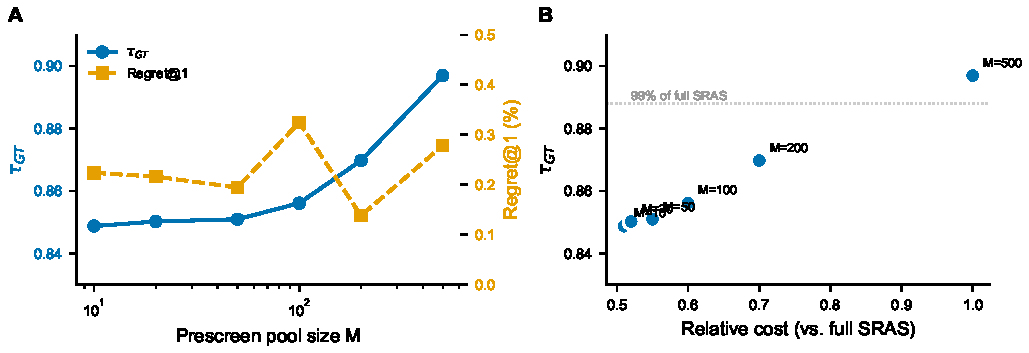
\includegraphics[width=\columnwidth]{fig12_two_stage.pdf}
\caption{Two-stage prescreening. \textbf{(A)} Performance vs.\ prescreen pool size $M$. \textbf{(B)} Cost-performance Pareto: $M = 50$--100 achieves $>$99\% of full \method{}'s $\taugt$ at $\sim$55--60\% cost.}
\label{fig:twostage}
\end{figure}

\subsection{Per-Architecture Variance}
\label{sec:variance}

Under the baseline, each architecture's rank fluctuates by 44.7 positions (std) across seeds; \method{} reduces this to 22.4 (\textbf{50\% reduction}). The improvement is largest for \textbf{top-performing architectures}: rank std drops from 31.3 to 11.3 (\textbf{64\% reduction})---precisely where stability matters most.

%% ======================================================================
%% 6. DISCUSSION
%% ======================================================================
\section{Discussion}
\label{sec:discussion}

\paragraph{Practical recipe.}
Based on our experiments, we recommend the following recipe for adopting \method{} (\Cref{tab:recipe}). The key insight is that $K = 3$ provides most of the gain at no extra training cost, while two-stage prescreening ($M = 50$) makes evaluation practical for large search spaces.

\begin{table}[t]
\centering
\caption{Practical \method{} recipe.}
\label{tab:recipe}
\small
\begin{tabular}{@{}lp{4.2cm}@{}}
\toprule
\textbf{Parameter} & \textbf{Recommendation} \\
\midrule
Warmup runs $K$ & 3--5 ($K{=}3$ at $1{\times}$ budget) \\
Warmup length $T_w$ & $T / K$ (budget parity) \\
Aggregation & Avg or z-score (equivalent) \\
BN recalib.\ & Recommended, not critical \\
Prescreening & Top-$M$, $M{=}50$--100 for large $N$ \\
Seed diversity & \textbf{Must} vary init, shuffle, aug \\
\midrule
\textbf{Report} & Median$\pm$IQR over ${\geq}3$ seeds \\
\bottomrule
\end{tabular}
\end{table}

\paragraph{Honest assessment: what z-score adds.}
Our ensemble baseline analysis (\Cref{sec:ensembles}) shows that simple averaging performs comparably to z-score normalization in homogeneous settings. Z-score's advantage is theoretical: it is scale-invariant when combining runs with heterogeneous training configurations. The practical contribution of \method{} is not a novel aggregation function, but the \textit{framework} of trading training depth for seed diversity under a fixed budget, supported by the empirical evidence that this trade-off is favorable.

\paragraph{Combining with training-time methods.}
\method{} is orthogonal to FairNAS~\cite{chu2021fairnas}, progressive shrinking~\cite{cai2020ofa}, and landmark regularization~\cite{yu2021landmark}. \method{} reduces seed noise; stabilization methods reduce training noise. Combining them should yield further gains.

\paragraph{Calibration gap.}
Our simulation uses $\taugt \approx 0.79$, more optimistic than published one-shot correlations of $0.3$--$0.5$~\cite{yu2020evaluating}. Our reported instability is therefore a \textit{lower bound}; real-world seed sensitivity is likely worse, making \method{} even more valuable in practice (\Cref{fig:tau_calibration}).

\begin{figure}[t]
\centering
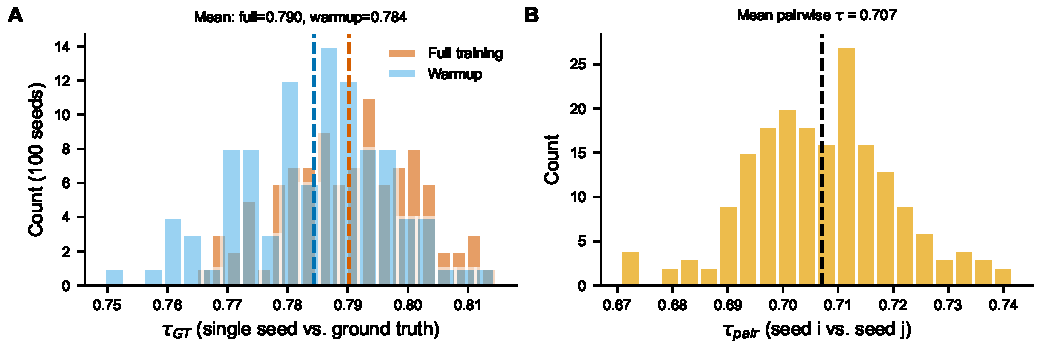
\includegraphics[width=\columnwidth]{fig13_tau_calibration.pdf}
\caption{Calibration sanity check. \textbf{(A)} Distribution of $\taugt$ across 100 seeds for full training (mean 0.790) and warmup (mean 0.784). \textbf{(B)} Pairwise $\taupair$ distribution (mean 0.707).}
\label{fig:tau_calibration}
\end{figure}

%% ======================================================================
%% 7. LIMITATIONS
%% ======================================================================
\section{Limitations}
\label{sec:limitations}

Our experiments use a calibrated simulation rather than actual supernet training. While calibrated to published values~\cite{yu2020evaluating,yang2020nas}, simulation cannot capture all training dynamics (optimizer coupling, DARTS collapse~\cite{zela2020robustdarts}, batch norm edge cases). Validation on real NAS-Bench-201 supernet training is needed to confirm improvement magnitudes.

We do not compare against training-time stabilization methods (e.g., landmark regularization~\cite{yu2021landmark}). Such a comparison, or a demonstration of combination gains, would strengthen the contribution.

We study only discrete one-shot search spaces. Extension to continuous relaxation (DARTS-style) is non-trivial and left for future work.

%% ======================================================================
%% 8. CONCLUSION
%% ======================================================================
\section{Conclusion}
\label{sec:conclusion}

Random seed sensitivity is a critical confounder in one-shot NAS: a single run produces rankings where top-5 overlap is only 29\% across seeds and 10 different ``best'' architectures are selected out of 20 runs. \method{}---multi-seed warmup with rank aggregation---raises pairwise $\tau$ by $+0.15$, top-5 overlap by $+40$pp, and cuts regret by $5.7\times$, all at equal compute budget. Our extensive ablations reveal that the primary driver is seed diversity (ensembling), not the specific normalization method; that BN recalibration is helpful but not essential; that noise reduction follows $K^{-0.45}$; and that a two-stage variant halves evaluation cost with minimal quality loss. \method{} is method-agnostic and can be adopted as a drop-in replacement for single-seed evaluation.

{
    \small
    \bibliographystyle{ieeenat_fullname}
    \bibliography{references}
}

\end{document}
